\documentclass[border=3pt,tikz]{standalone}
\usepackage{amsmath} 
\usetikzlibrary{arrows.meta} 
\usetikzlibrary{fit, positioning, backgrounds, scopes} 
\usepackage[outline]{contour} 
\contourlength{1.4pt}

% COLORS
\usepackage{xcolor}
\colorlet{myred}{red!80!black}
\colorlet{myblue}{blue!80!black}
\colorlet{mygreen}{green!60!black}
\colorlet{myorange}{orange!70!red!60!black}
\colorlet{mydarkred}{red!30!black}
\colorlet{mydarkblue}{blue!40!black}
\colorlet{mydarkgreen}{green!30!black}

% STYLES
\tikzset{
  >=latex, 
  node/.style={thick,circle,draw=myblue,minimum size=20,inner sep=0.5,outer sep=0.6},
  node in/.style={node,green!20!black,draw=mygreen!30!black,fill=mygreen!25},
  node trunk/.style={node,blue!20!black,draw=myblue!30!black,fill=myblue!20},
  node head/.style={node,orange!20!black,draw=myorange!30!black,fill=myorange!20},
  node out/.style={node,red!20!black,draw=myred!30!black,fill=myred!20},
  connect/.style={thick,mydarkblue},
  label/.style={font=\small,align=center},
  box/.style={draw, thick, rounded corners, inner sep=10pt, fill opacity=0.05}
}

\begin{document}

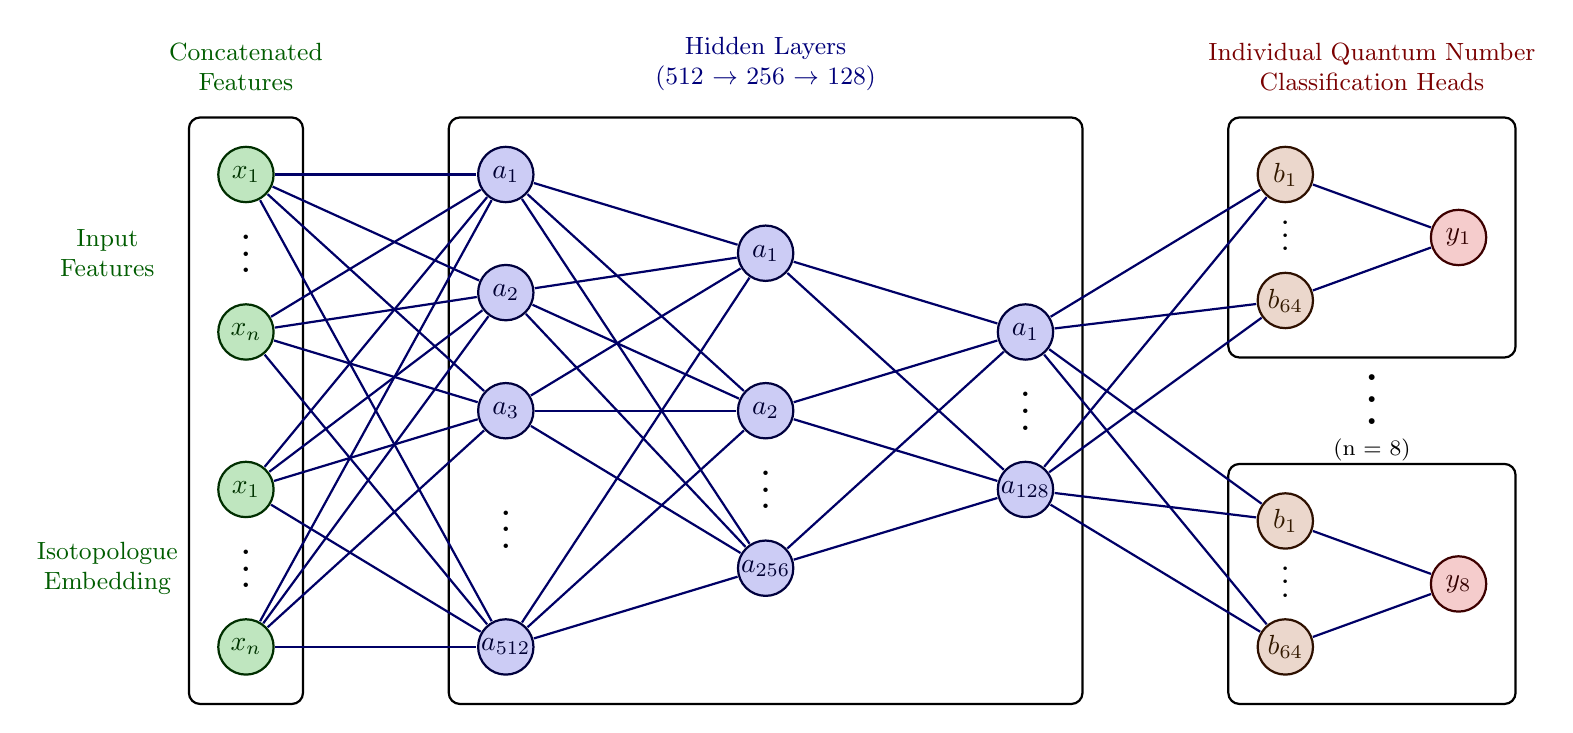
\begin{tikzpicture}[x=2.2cm,y=1.0cm]
  
  % --- LAYER 1: INPUTS (x=1) ---
  % Group 1: Input Features 
  \node[node in] (N1-1) at (1, 3) {$x_1$};
  \node[node in] (N1-2) at (1, 1) {$x_n$};
  \path (N1-1) -- (N1-2) node[pos=0.5, yshift=0.15cm, scale=1.5] {$\vdots$};

  % Group 2: Isotopologue Embedding
  \node[node in] (N1-i1) at (1, -1) {$x_1$};
  \node[node in] (N1-i2) at (1, -3) {$x_n$};
  \path (N1-i1) -- (N1-i2) node[pos=0.5, yshift=0.15cm, scale=1.5] {$\vdots$};

  \begin{pgfonlayer}{background}
    \node[box, fit=(N1-1) (N1-i2), fill=mygreen!3] (input-box) {}; 
  \end{pgfonlayer}

  \node[label, mygreen!60!black] at (0.2, 2) {Input\\Features}; 
  \node[label, mygreen!60!black] at (0.2, -2) {Isotopologue\\Embedding}; 
  \node[label, mygreen!60!black, above=2mm of input-box.north] {Concatenated\\Features}; 

  % --- LAYER 2: TRUNK (512 -> 256 -> 128) ---
  % 512 Nodes (3+1)
  \node[node trunk] (N2-1) at (2.5, 3) {$a_1$};
  \node[node trunk] (N2-2) at (2.5, 1.5) {$a_2$};
  \node[node trunk] (N2-3) at (2.5, 0) {$a_3$};
  \node[node trunk] (N2-4) at (2.5, -3) {$a_{512}$};
  \path (N2-3) -- (N2-4) node[pos=0.5, yshift=0.15cm, scale=1.5] {$\vdots$};
  
  % 256 Nodes (2+1)
  \node[node trunk] (N3-1) at (4, 2) {$a_1$};
  \node[node trunk] (N3-2) at (4, 0) {$a_2$};
  \node[node trunk] (N3-3) at (4, -2) {$a_{256}$};
  \path (N3-2) -- (N3-3) node[pos=0.5, yshift=0.15cm, scale=1.5] {$\vdots$};

  % 128 Nodes (1+1)
  \node[node trunk] (N4-1) at (5.5, 1) {$a_1$};
  \node[node trunk] (N4-2) at (5.5, -1) {$a_{128}$};
  \path (N4-1) -- (N4-2) node[pos=0.5, yshift=0.15cm, scale=1.5] {$\vdots$};
  
  % Connections Trunk 
  \foreach \i in {N1-1,N1-2,N1-i1,N1-i2} \foreach \j in {1,2,3,4} \draw[connect] (\i) -- (N2-\j);
  \foreach \i in {1,2,3,4} \foreach \j in {1,2,3} \draw[connect] (N2-\i) -- (N3-\j);
  \foreach \i in {1,2,3} \foreach \j in {1,2} \draw[connect] (N3-\i) -- (N4-\j);
  
  \begin{pgfonlayer}{background}
    \node[box, fit=(N2-1) (N2-4) (N4-2), fill=myblue!3] (trunk-box) {}; 
  \end{pgfonlayer}
  \node[label, myblue!60!black, above=2mm of trunk-box.north] {Hidden Layers\\(512 $\to$ 256 $\to$ 128)}; 

  % --- LAYER 3: ADAPTER HEADS ---
  % Head 1 
  \begin{scope}[yshift=2.2cm]
    \node[node head] (H1-1) at (7, 0.8) {$b_1$}; 
    \node[node head] (H1-2) at (7, -0.8) {$b_{64}$}; 
    \path (H1-1) -- (H1-2) node[pos=0.5, yshift=0.15cm, scale=1.2] {$\vdots$};
    \node[node out] (O1) at (8, 0) {$y_1$}; 
    \foreach \i in {1,2} \foreach \j in {1,2} \draw[connect] (N4-\i) -- (H1-\j); 
    \foreach \i in {1,2} \draw[connect] (H1-\i) -- (O1); 
    \begin{pgfonlayer}{background}
      \node[box, fit=(H1-1) (O1) (H1-2), fill=myorange!3] (head1-box) {}; 
    \end{pgfonlayer}
  \end{scope}

  % Global \vdots between heads, visually centered at y=0, shifted up to clear text
  \node[scale=2.0] at (7.5, 0.35) {$\vdots$}; 
  \node[label, font=\footnotesize] at (7.5, -0.5) {(n = 8)};

  % Head 8 
  \begin{scope}[yshift=-2.2cm]
    \node[node head] (H8-1) at (7, 0.8) {$b_1$}; 
    \node[node head] (H8-2) at (7, -0.8) {$b_{64}$}; 
    \path (H8-1) -- (H8-2) node[pos=0.5, yshift=0.15cm, scale=1.2] {$\vdots$};
    \node[node out] (O8) at (8, 0) {$y_8$}; 
    \foreach \i in {1,2} \foreach \j in {1,2} \draw[connect] (N4-\i) -- (H8-\j); 
    \foreach \i in {1,2} \draw[connect] (H8-\i) -- (O8); 
    \begin{pgfonlayer}{background}
      \node[box, fit=(H8-1) (O8) (H8-2), fill=myorange!3] (head8-box) {}; 
    \end{pgfonlayer}
  \end{scope}
  
  \node[label, myred!60!black, above=2mm of head1-box.north] {Individual Quantum Number\\Classification Heads};

\end{tikzpicture}
\end{document}